\documentclass[1p]{elsarticle_modified}
%\bibliographystyle{elsarticle-num}

%\usepackage[colorlinks]{hyperref}
%\usepackage{abbrmath_seonhwa} %\Abb, \Ascr, \Acal ,\Abf, \Afrak
\usepackage{amsfonts}
\usepackage{amssymb}
\usepackage{amsmath}
\usepackage{amsthm}
\usepackage{scalefnt}
\usepackage{amsbsy}
\usepackage{kotex}
\usepackage{caption}
\usepackage{subfig}
\usepackage{color}
\usepackage{graphicx}
\usepackage{xcolor} %% white, black, red, green, blue, cyan, magenta, yellow
\usepackage{float}
\usepackage{setspace}
\usepackage{hyperref}

\usepackage{tikz}
\usetikzlibrary{arrows}

\usepackage{multirow}
\usepackage{array} % fixed length table
\usepackage{hhline}

%%%%%%%%%%%%%%%%%%%%%
\makeatletter
\renewcommand*\env@matrix[1][\arraystretch]{%
	\edef\arraystretch{#1}%
	\hskip -\arraycolsep
	\let\@ifnextchar\new@ifnextchar
	\array{*\c@MaxMatrixCols c}}
\makeatother %https://tex.stackexchange.com/questions/14071/how-can-i-increase-the-line-spacing-in-a-matrix
%%%%%%%%%%%%%%%

\usepackage[normalem]{ulem}

\newcommand{\msout}[1]{\ifmmode\text{\sout{\ensuremath{#1}}}\else\sout{#1}\fi}
%SOURCE: \msout is \stkout macro in https://tex.stackexchange.com/questions/20609/strikeout-in-math-mode

\newcommand{\cancel}[1]{
	\ifmmode
	{\color{red}\msout{#1}}
	\else
	{\color{red}\sout{#1}}
	\fi
}

\newcommand{\add}[1]{
	{\color{blue}\uwave{#1}}
}

\newcommand{\replace}[2]{
	\ifmmode
	{\color{red}\msout{#1}}{\color{blue}\uwave{#2}}
	\else
	{\color{red}\sout{#1}}{\color{blue}\uwave{#2}}
	\fi
}

\newcommand{\Sol}{\mathcal{S}} %segment
\newcommand{\D}{D} %diagram
\newcommand{\A}{\mathcal{A}} %arc


%%%%%%%%%%%%%%%%%%%%%%%%%%%%%5 test

\def\sl{\operatorname{\textup{SL}}(2,\Cbb)}
\def\psl{\operatorname{\textup{PSL}}(2,\Cbb)}
\def\quan{\mkern 1mu \triangleright \mkern 1mu}

\theoremstyle{definition}
\newtheorem{thm}{Theorem}[section]
\newtheorem{prop}[thm]{Proposition}
\newtheorem{lem}[thm]{Lemma}
\newtheorem{ques}[thm]{Question}
\newtheorem{cor}[thm]{Corollary}
\newtheorem{defn}[thm]{Definition}
\newtheorem{exam}[thm]{Example}
\newtheorem{rmk}[thm]{Remark}
\newtheorem{alg}[thm]{Algorithm}

\newcommand{\I}{\sqrt{-1}}
\begin{document}

%\begin{frontmatter}
%
%\title{Boundary parabolic representations of knots up to 8 crossings}
%
%%% Group authors per affiliation:
%\author{Yunhi Cho} 
%\address{Department of Mathematics, University of Seoul, Seoul, Korea}
%\ead{yhcho@uos.ac.kr}
%
%
%\author{Seonhwa Kim} %\fnref{s_kim}}
%\address{Center for Geometry and Physics, Institute for Basic Science, Pohang, 37673, Korea}
%\ead{ryeona17@ibs.re.kr}
%
%\author{Hyuk Kim}
%\address{Department of Mathematical Sciences, Seoul National University, Seoul 08826, Korea}
%\ead{hyukkim@snu.ac.kr}
%
%\author{Seokbeom Yoon}
%\address{Department of Mathematical Sciences, Seoul National University, Seoul, 08826,  Korea}
%\ead{sbyoon15@snu.ac.kr}
%
%\begin{abstract}
%We find all boundary parabolic representation of knots up to 8 crossings.
%
%\end{abstract}
%\begin{keyword}
%    \MSC[2010] 57M25 
%\end{keyword}
%
%\end{frontmatter}

%\linenumbers
%\tableofcontents
%
\newcommand\colored[1]{\textcolor{white}{\rule[-0.35ex]{0.8em}{1.4ex}}\kern-0.8em\color{red} #1}%
%\newcommand\colored[1]{\textcolor{white}{ #1}\kern-2.17ex	\textcolor{white}{ #1}\kern-1.81ex	\textcolor{white}{ #1}\kern-2.15ex\color{red}#1	}

{\Large $\underline{12n_{0699}~(K12n_{0699})}$}

\setlength{\tabcolsep}{10pt}
\renewcommand{\arraystretch}{1.6}
\vspace{1cm}\begin{tabular}{m{100pt}>{\centering\arraybackslash}m{274pt}}
\multirow{5}{120pt}{
	\centering
	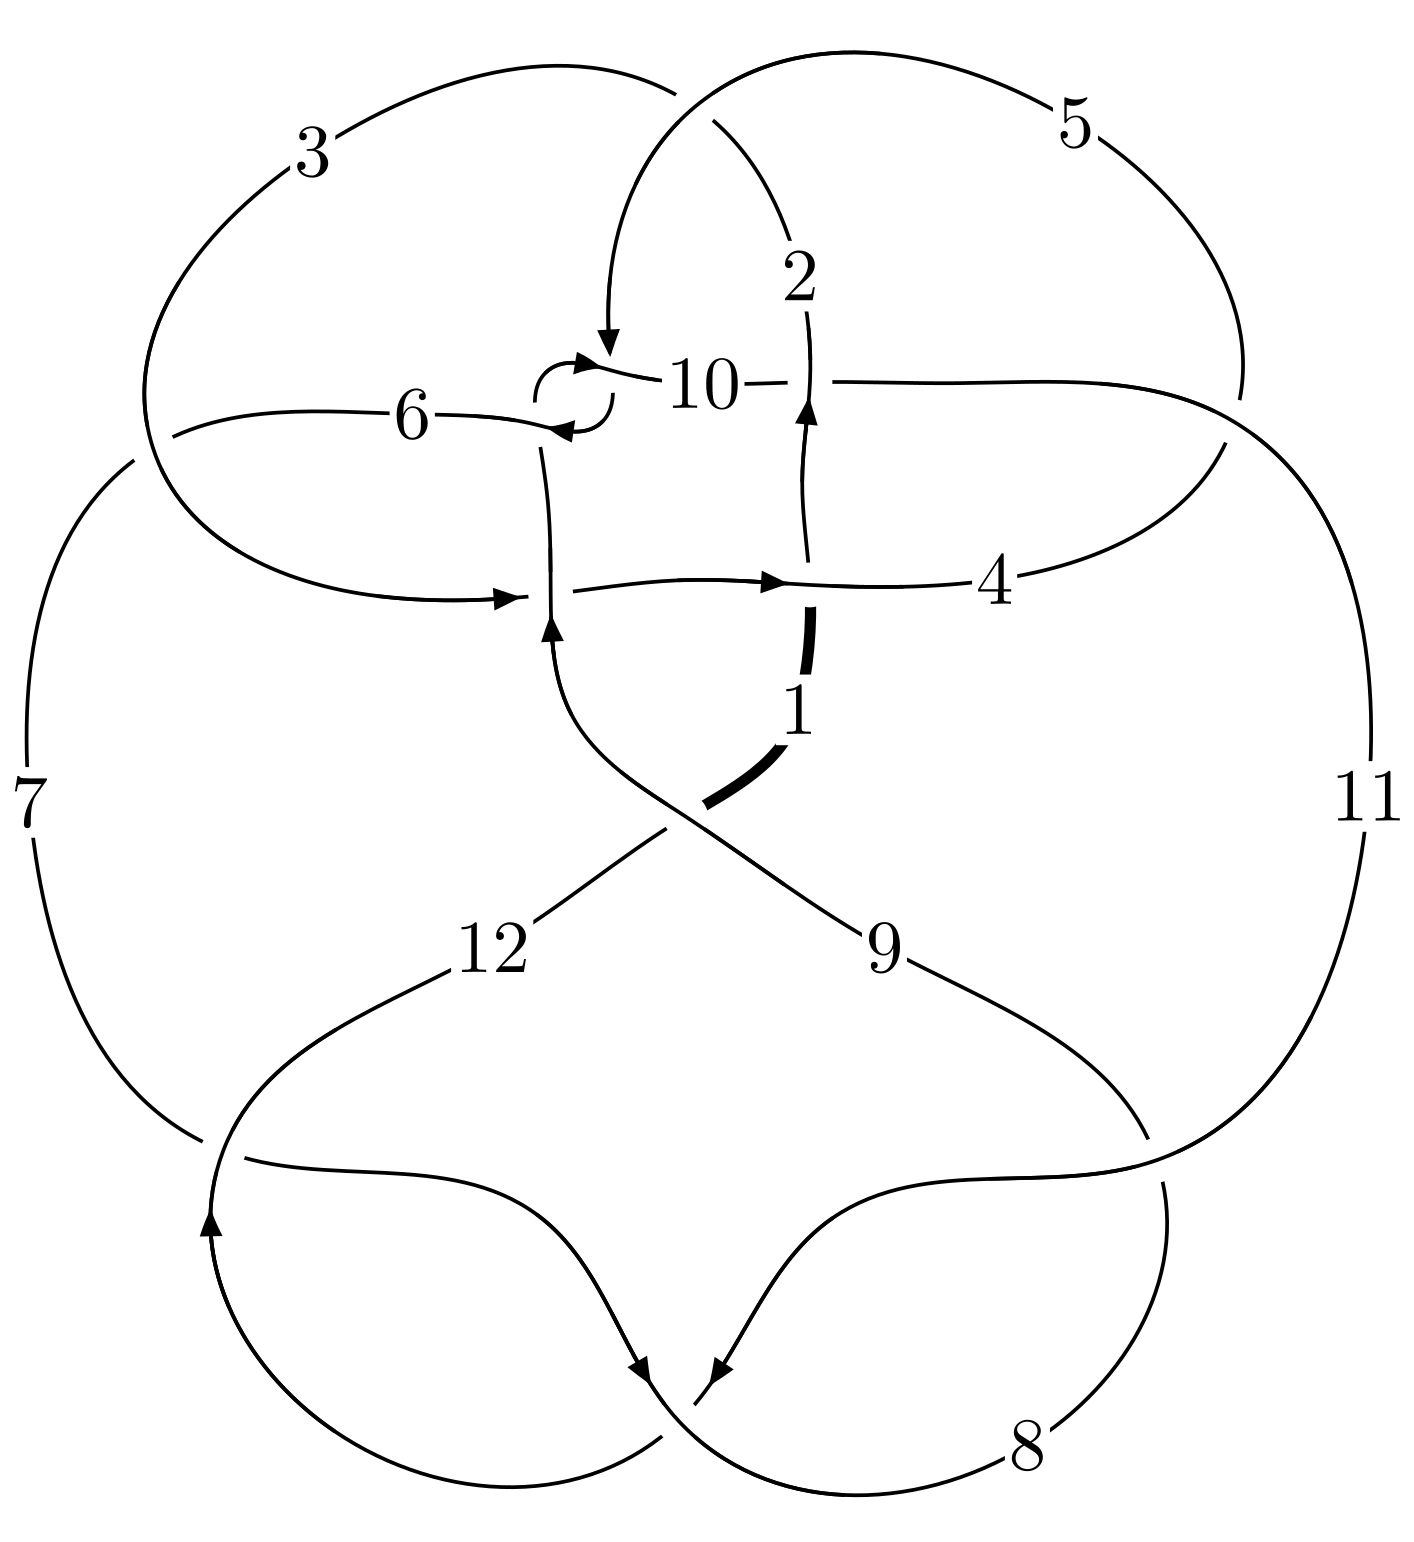
\includegraphics[width=112pt]{../../../GIT/diagram.site/Diagrams/png/2788_12n_0699.png}\\
\ \ \ A knot diagram\footnotemark}&
\allowdisplaybreaks
\textbf{Linearized knot diagam} \\
\cline{2-2}
 &
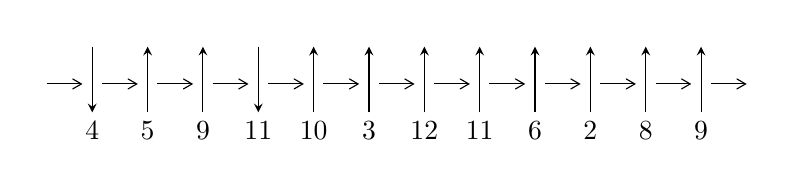
\begin{tikzpicture}[x=20pt, y=17pt]
	% nodes
	\node (C0) at (0, 0) {};
	\node (C1) at (1, 0) {};
	\node (C1U) at (1, +1) {};
	\node (C1D) at (1, -1) {4};

	\node (C2) at (2, 0) {};
	\node (C2U) at (2, +1) {};
	\node (C2D) at (2, -1) {5};

	\node (C3) at (3, 0) {};
	\node (C3U) at (3, +1) {};
	\node (C3D) at (3, -1) {9};

	\node (C4) at (4, 0) {};
	\node (C4U) at (4, +1) {};
	\node (C4D) at (4, -1) {11};

	\node (C5) at (5, 0) {};
	\node (C5U) at (5, +1) {};
	\node (C5D) at (5, -1) {10};

	\node (C6) at (6, 0) {};
	\node (C6U) at (6, +1) {};
	\node (C6D) at (6, -1) {3};

	\node (C7) at (7, 0) {};
	\node (C7U) at (7, +1) {};
	\node (C7D) at (7, -1) {12};

	\node (C8) at (8, 0) {};
	\node (C8U) at (8, +1) {};
	\node (C8D) at (8, -1) {11};

	\node (C9) at (9, 0) {};
	\node (C9U) at (9, +1) {};
	\node (C9D) at (9, -1) {6};

	\node (C10) at (10, 0) {};
	\node (C10U) at (10, +1) {};
	\node (C10D) at (10, -1) {2};

	\node (C11) at (11, 0) {};
	\node (C11U) at (11, +1) {};
	\node (C11D) at (11, -1) {8};

	\node (C12) at (12, 0) {};
	\node (C12U) at (12, +1) {};
	\node (C12D) at (12, -1) {9};
	\node (C13) at (13, 0) {};

	% arrows
	\draw[->,>={angle 60}]
	(C0) edge (C1) (C1) edge (C2) (C2) edge (C3) (C3) edge (C4) (C4) edge (C5) (C5) edge (C6) (C6) edge (C7) (C7) edge (C8) (C8) edge (C9) (C9) edge (C10) (C10) edge (C11) (C11) edge (C12) (C12) edge (C13) ;	\draw[->,>=stealth]
	(C1U) edge (C1D) (C2D) edge (C2U) (C3D) edge (C3U) (C4U) edge (C4D) (C5D) edge (C5U) (C6D) edge (C6U) (C7D) edge (C7U) (C8D) edge (C8U) (C9D) edge (C9U) (C10D) edge (C10U) (C11D) edge (C11U) (C12D) edge (C12U) ;
	\end{tikzpicture} \\
\hhline{~~} \\& 
\textbf{Solving Sequence} \\ \cline{2-2} 
 &
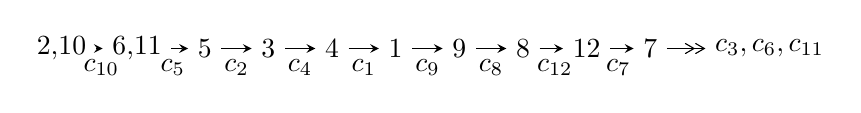
\begin{tikzpicture}[x=23pt, y=7pt]
	% node
	\node (A0) at (-1/8, 0) {2,10};
	\node (A1) at (17/16, 0) {6,11};
	\node (A2) at (17/8, 0) {5};
	\node (A3) at (25/8, 0) {3};
	\node (A4) at (33/8, 0) {4};
	\node (A5) at (41/8, 0) {1};
	\node (A6) at (49/8, 0) {9};
	\node (A7) at (57/8, 0) {8};
	\node (A8) at (65/8, 0) {12};
	\node (A9) at (73/8, 0) {7};
	\node (C1) at (1/2, -1) {$c_{10}$};
	\node (C2) at (13/8, -1) {$c_{5}$};
	\node (C3) at (21/8, -1) {$c_{2}$};
	\node (C4) at (29/8, -1) {$c_{4}$};
	\node (C5) at (37/8, -1) {$c_{1}$};
	\node (C6) at (45/8, -1) {$c_{9}$};
	\node (C7) at (53/8, -1) {$c_{8}$};
	\node (C8) at (61/8, -1) {$c_{12}$};
	\node (C9) at (69/8, -1) {$c_{7}$};
	\node (A10) at (11, 0) {$c_{3},c_{6},c_{11}$};

	% edge
	\draw[->,>=stealth]	
	(A0) edge (A1) (A1) edge (A2) (A2) edge (A3) (A3) edge (A4) (A4) edge (A5) (A5) edge (A6) (A6) edge (A7) (A7) edge (A8) (A8) edge (A9) ;
	\draw[->>,>={angle 60}]	
	(A9) edge (A10);
\end{tikzpicture} \\ 

\end{tabular} \\

\footnotetext{
The image of knot diagram is generated by the software ``\textbf{Draw programme}" developed by Andrew Bartholomew(\url{http://www.layer8.co.uk/maths/draw/index.htm\#Running-draw}), where we modified some parts for our purpose(\url{https://github.com/CATsTAILs/LinksPainter}).
}\phantom \\ \newline 
\centering \textbf{Ideals for irreducible components\footnotemark of $X_{\text{par}}$} 
 
\begin{align*}
I^u_{1}&=\langle 
-4.48533\times10^{64} u^{38}-1.99110\times10^{65} u^{37}+\cdots+1.70583\times10^{66} b+7.99429\times10^{65},\\
\phantom{I^u_{1}}&\phantom{= \langle  }2.92714\times10^{66} u^{38}+1.55651\times10^{67} u^{37}+\cdots+4.94689\times10^{67} a+4.66164\times10^{68},\;u^{39}+4 u^{38}+\cdots+95 u+29\rangle \\
I^u_{2}&=\langle 
-206 u^{15}+554 u^{14}+\cdots+239 b+200,\;-339 u^{15}+914 u^{14}+\cdots+239 a+53,\\
\phantom{I^u_{2}}&\phantom{= \langle  }u^{16}-3 u^{15}+5 u^{14}-4 u^{13}+3 u^{12}-6 u^{11}+12 u^{10}-10 u^9+u^8+6 u^7-3 u^5+2 u^4+3 u^3- u+1\rangle \\
\\
\end{align*}
\raggedright * 2 irreducible components of $\dim_{\mathbb{C}}=0$, with total 55 representations.\\
\footnotetext{All coefficients of polynomials are rational numbers. But the coefficients are sometimes approximated in decimal forms when there is not enough margin.}
\newpage
\renewcommand{\arraystretch}{1}
\centering \section*{I. $I^u_{1}= \langle -4.49\times10^{64} u^{38}-1.99\times10^{65} u^{37}+\cdots+1.71\times10^{66} b+7.99\times10^{65},\;2.93\times10^{66} u^{38}+1.56\times10^{67} u^{37}+\cdots+4.95\times10^{67} a+4.66\times10^{68},\;u^{39}+4 u^{38}+\cdots+95 u+29 \rangle$}
\flushleft \textbf{(i) Arc colorings}\\
\begin{tabular}{m{7pt} m{180pt} m{7pt} m{180pt} }
\flushright $a_{2}=$&$\begin{pmatrix}0\\u\end{pmatrix}$ \\
\flushright $a_{10}=$&$\begin{pmatrix}1\\0\end{pmatrix}$ \\
\flushright $a_{6}=$&$\begin{pmatrix}-0.0591713 u^{38}-0.314643 u^{37}+\cdots-24.3274 u-9.42337\\0.0262942 u^{38}+0.116723 u^{37}+\cdots+4.56393 u-0.468647\end{pmatrix}$ \\
\flushright $a_{11}=$&$\begin{pmatrix}1\\- u^2\end{pmatrix}$ \\
\flushright $a_{5}=$&$\begin{pmatrix}-0.0854656 u^{38}-0.431367 u^{37}+\cdots-28.8913 u-8.95473\\0.0262942 u^{38}+0.116723 u^{37}+\cdots+4.56393 u-0.468647\end{pmatrix}$ \\
\flushright $a_{3}=$&$\begin{pmatrix}0.517557 u^{38}+2.13119 u^{37}+\cdots+67.6443 u+17.6022\\0.128326 u^{38}+0.499772 u^{37}+\cdots+14.8366 u+3.04010\end{pmatrix}$ \\
\flushright $a_{4}=$&$\begin{pmatrix}0.0201548 u^{38}-0.000488821 u^{37}+\cdots-13.3460 u-6.82775\\0.0712460 u^{38}+0.287520 u^{37}+\cdots+8.42457 u-0.225151\end{pmatrix}$ \\
\flushright $a_{1}=$&$\begin{pmatrix}0.120505 u^{38}+0.724667 u^{37}+\cdots+51.9973 u+19.7269\\-0.0193862 u^{38}+0.0323405 u^{37}+\cdots+18.8628 u+7.88916\end{pmatrix}$ \\
\flushright $a_{9}=$&$\begin{pmatrix}-0.170703 u^{38}-0.565196 u^{37}+\cdots-9.52828 u+2.61870\\-0.0658720 u^{38}-0.274198 u^{37}+\cdots-13.3540 u-2.25891\end{pmatrix}$ \\
\flushright $a_{8}=$&$\begin{pmatrix}-0.108782 u^{38}-0.236844 u^{37}+\cdots+10.0488 u+8.28847\\-0.00548525 u^{38}-0.0123701 u^{37}+\cdots-3.89489 u+0.0804277\end{pmatrix}$ \\
\flushright $a_{12}=$&$\begin{pmatrix}-0.406322 u^{38}-1.94808 u^{37}+\cdots-100.418 u-28.6038\\-0.156580 u^{38}-0.684622 u^{37}+\cdots-24.5158 u-6.19127\end{pmatrix}$ \\
\flushright $a_{7}=$&$\begin{pmatrix}0.518418 u^{38}+1.72726 u^{37}+\cdots+17.1390 u-6.89267\\0.124927 u^{38}+0.415220 u^{37}+\cdots-0.251870 u-2.53467\end{pmatrix}$\\&\end{tabular}
\flushleft \textbf{(ii) Obstruction class $= -1$}\\~\\
\flushleft \textbf{(iii) Cusp Shapes $= -0.432519 u^{38}-1.98528 u^{37}+\cdots-85.2061 u-12.7504$}\\~\\
\newpage\renewcommand{\arraystretch}{1}
\flushleft \textbf{(iv) u-Polynomials at the component}\newline \\
\begin{tabular}{m{50pt}|m{274pt}}
Crossings & \hspace{64pt}u-Polynomials at each crossing \\
\hline $$\begin{aligned}c_{1}\end{aligned}$$&$\begin{aligned}
&u^{39}+6 u^{38}+\cdots+68813 u-4453
\end{aligned}$\\
\hline $$\begin{aligned}c_{2}\end{aligned}$$&$\begin{aligned}
&u^{39}+12 u^{38}+\cdots+33 u-1
\end{aligned}$\\
\hline $$\begin{aligned}c_{3}\end{aligned}$$&$\begin{aligned}
&u^{39}- u^{38}+\cdots-7950 u-6379
\end{aligned}$\\
\hline $$\begin{aligned}c_{4}\end{aligned}$$&$\begin{aligned}
&u^{39}-17 u^{37}+\cdots+59051 u-25039
\end{aligned}$\\
\hline $$\begin{aligned}c_{5},c_{9}\end{aligned}$$&$\begin{aligned}
&u^{39}-3 u^{38}+\cdots-8 u-1
\end{aligned}$\\
\hline $$\begin{aligned}c_{6}\end{aligned}$$&$\begin{aligned}
&u^{39}-4 u^{38}+\cdots+621578 u-106361
\end{aligned}$\\
\hline $$\begin{aligned}c_{7},c_{8},c_{11}\end{aligned}$$&$\begin{aligned}
&u^{39}+u^{38}+\cdots+40 u-13
\end{aligned}$\\
\hline $$\begin{aligned}c_{10}\end{aligned}$$&$\begin{aligned}
&u^{39}-4 u^{38}+\cdots+95 u-29
\end{aligned}$\\
\hline $$\begin{aligned}c_{12}\end{aligned}$$&$\begin{aligned}
&u^{39}- u^{38}+\cdots+1387526 u-100009
\end{aligned}$\\
\hline
\end{tabular}\\~\\
\newpage\renewcommand{\arraystretch}{1}
\flushleft \textbf{(v) Riley Polynomials at the component}\newline \\
\begin{tabular}{m{50pt}|m{274pt}}
Crossings & \hspace{64pt}Riley Polynomials at each crossing \\
\hline $$\begin{aligned}c_{1}\end{aligned}$$&$\begin{aligned}
&y^{39}-86 y^{38}+\cdots+1745564923 y-19829209
\end{aligned}$\\
\hline $$\begin{aligned}c_{2}\end{aligned}$$&$\begin{aligned}
&y^{39}+12 y^{38}+\cdots+2135 y-1
\end{aligned}$\\
\hline $$\begin{aligned}c_{3}\end{aligned}$$&$\begin{aligned}
&y^{39}+77 y^{38}+\cdots-133130362 y-40691641
\end{aligned}$\\
\hline $$\begin{aligned}c_{4}\end{aligned}$$&$\begin{aligned}
&y^{39}-34 y^{38}+\cdots+7818316899 y-626951521
\end{aligned}$\\
\hline $$\begin{aligned}c_{5},c_{9}\end{aligned}$$&$\begin{aligned}
&y^{39}+31 y^{38}+\cdots+48 y-1
\end{aligned}$\\
\hline $$\begin{aligned}c_{6}\end{aligned}$$&$\begin{aligned}
&y^{39}+52 y^{38}+\cdots+161820928428 y-11312662321
\end{aligned}$\\
\hline $$\begin{aligned}c_{7},c_{8},c_{11}\end{aligned}$$&$\begin{aligned}
&y^{39}+61 y^{38}+\cdots-4614 y-169
\end{aligned}$\\
\hline $$\begin{aligned}c_{10}\end{aligned}$$&$\begin{aligned}
&y^{39}+12 y^{38}+\cdots-9187 y-841
\end{aligned}$\\
\hline $$\begin{aligned}c_{12}\end{aligned}$$&$\begin{aligned}
&y^{39}+199 y^{38}+\cdots-836738153944 y-10001800081
\end{aligned}$\\
\hline
\end{tabular}\\~\\
\newpage\flushleft \textbf{(vi) Complex Volumes and Cusp Shapes}
$$\begin{array}{c|c|c}  
\text{Solutions to }I^u_{1}& \I (\text{vol} + \sqrt{-1}CS) & \text{Cusp shape}\\
 \hline 
\begin{aligned}
u &= \phantom{-}0.443892 + 0.894212 I \\
a &= \phantom{-}0.136058 - 0.043126 I \\
b &= \phantom{-}1.102760 + 0.179428 I\end{aligned}
 & -4.34392 + 3.40044 I & \phantom{-}2.15847 - 4.15591 I \\ \hline\begin{aligned}
u &= \phantom{-}0.443892 - 0.894212 I \\
a &= \phantom{-}0.136058 + 0.043126 I \\
b &= \phantom{-}1.102760 - 0.179428 I\end{aligned}
 & -4.34392 - 3.40044 I & \phantom{-}2.15847 + 4.15591 I \\ \hline\begin{aligned}
u &= \phantom{-}0.584880 + 0.814792 I \\
a &= \phantom{-}1.18601 - 1.16107 I \\
b &= -0.391017 - 1.238900 I\end{aligned}
 & -2.68089 + 4.77988 I & \phantom{-}0.54174 - 3.58018 I \\ \hline\begin{aligned}
u &= \phantom{-}0.584880 - 0.814792 I \\
a &= \phantom{-}1.18601 + 1.16107 I \\
b &= -0.391017 + 1.238900 I\end{aligned}
 & -2.68089 - 4.77988 I & \phantom{-}0.54174 + 3.58018 I \\ \hline\begin{aligned}
u &= \phantom{-}0.388962 + 0.964036 I \\
a &= -0.68810 + 1.25836 I \\
b &= \phantom{-}0.080712 + 1.199870 I\end{aligned}
 & -3.44253 - 0.59700 I & \phantom{-}4.34930 + 3.15252 I \\ \hline\begin{aligned}
u &= \phantom{-}0.388962 - 0.964036 I \\
a &= -0.68810 - 1.25836 I \\
b &= \phantom{-}0.080712 - 1.199870 I\end{aligned}
 & -3.44253 + 0.59700 I & \phantom{-}4.34930 - 3.15252 I \\ \hline\begin{aligned}
u &= \phantom{-}0.724071 + 0.767036 I \\
a &= \phantom{-}0.527790 + 0.780046 I \\
b &= \phantom{-}0.123047 + 0.078516 I\end{aligned}
 & -3.74668 + 1.00507 I & \phantom{-}3.79526 - 1.05866 I \\ \hline\begin{aligned}
u &= \phantom{-}0.724071 - 0.767036 I \\
a &= \phantom{-}0.527790 - 0.780046 I \\
b &= \phantom{-}0.123047 - 0.078516 I\end{aligned}
 & -3.74668 - 1.00507 I & \phantom{-}3.79526 + 1.05866 I \\ \hline\begin{aligned}
u &= -0.181436 + 0.922500 I \\
a &= -0.74681 - 1.43570 I \\
b &= \phantom{-}0.57246 - 1.38204 I\end{aligned}
 & -8.18165 - 2.82026 I & -0.23535 + 2.51294 I \\ \hline\begin{aligned}
u &= -0.181436 - 0.922500 I \\
a &= -0.74681 + 1.43570 I \\
b &= \phantom{-}0.57246 + 1.38204 I\end{aligned}
 & -8.18165 + 2.82026 I & -0.23535 - 2.51294 I\\
 \hline 
 \end{array}$$\newpage$$\begin{array}{c|c|c}  
\text{Solutions to }I^u_{1}& \I (\text{vol} + \sqrt{-1}CS) & \text{Cusp shape}\\
 \hline 
\begin{aligned}
u &= -0.215429 + 1.104370 I \\
a &= \phantom{-}0.271873 - 1.261790 I \\
b &= -0.70054 - 1.42784 I\end{aligned}
 & \phantom{-}19.5709 - 0.0915 I & -0.041291 + 0.250584 I \\ \hline\begin{aligned}
u &= -0.215429 - 1.104370 I \\
a &= \phantom{-}0.271873 + 1.261790 I \\
b &= -0.70054 + 1.42784 I\end{aligned}
 & \phantom{-}19.5709 + 0.0915 I & -0.041291 - 0.250584 I \\ \hline\begin{aligned}
u &= \phantom{-}0.869795 + 0.024295 I \\
a &= \phantom{-}0.313165 + 0.718063 I \\
b &= \phantom{-}0.524688 + 0.787160 I\end{aligned}
 & -3.32799 + 1.95686 I & \phantom{-}7.87158 - 4.03984 I \\ \hline\begin{aligned}
u &= \phantom{-}0.869795 - 0.024295 I \\
a &= \phantom{-}0.313165 - 0.718063 I \\
b &= \phantom{-}0.524688 - 0.787160 I\end{aligned}
 & -3.32799 - 1.95686 I & \phantom{-}7.87158 + 4.03984 I \\ \hline\begin{aligned}
u &= -0.567289 + 0.618604 I \\
a &= -0.642417 + 0.111976 I \\
b &= \phantom{-}0.429754 + 0.191974 I\end{aligned}
 & \phantom{-}0.70753 - 1.66098 I & \phantom{-}4.28580 + 6.70295 I \\ \hline\begin{aligned}
u &= -0.567289 - 0.618604 I \\
a &= -0.642417 - 0.111976 I \\
b &= \phantom{-}0.429754 - 0.191974 I\end{aligned}
 & \phantom{-}0.70753 + 1.66098 I & \phantom{-}4.28580 - 6.70295 I \\ \hline\begin{aligned}
u &= -0.958602 + 0.745202 I \\
a &= -0.176071 + 1.110370 I \\
b &= -0.507024 - 0.126186 I\end{aligned}
 & -14.7115 + 0.6008 I & \phantom{-}6.01609 + 0.22717 I \\ \hline\begin{aligned}
u &= -0.958602 - 0.745202 I \\
a &= -0.176071 - 1.110370 I \\
b &= -0.507024 + 0.126186 I\end{aligned}
 & -14.7115 - 0.6008 I & \phantom{-}6.01609 - 0.22717 I \\ \hline\begin{aligned}
u &= -0.016312 + 0.768909 I \\
a &= \phantom{-}1.61762 + 2.88519 I \\
b &= \phantom{-}0.085474 + 1.237340 I\end{aligned}
 & -7.68184 + 2.01879 I & -2.91621 - 3.56990 I \\ \hline\begin{aligned}
u &= -0.016312 - 0.768909 I \\
a &= \phantom{-}1.61762 - 2.88519 I \\
b &= \phantom{-}0.085474 - 1.237340 I\end{aligned}
 & -7.68184 - 2.01879 I & -2.91621 + 3.56990 I\\
 \hline 
 \end{array}$$\newpage$$\begin{array}{c|c|c}  
\text{Solutions to }I^u_{1}& \I (\text{vol} + \sqrt{-1}CS) & \text{Cusp shape}\\
 \hline 
\begin{aligned}
u &= -0.202386 + 0.647908 I \\
a &= -0.94963 + 5.33367 I \\
b &= -0.170246 + 1.217870 I\end{aligned}
 & -17.9862 - 1.8167 I & -3.56636 + 4.57014 I \\ \hline\begin{aligned}
u &= -0.202386 - 0.647908 I \\
a &= -0.94963 - 5.33367 I \\
b &= -0.170246 - 1.217870 I\end{aligned}
 & -17.9862 + 1.8167 I & -3.56636 - 4.57014 I \\ \hline\begin{aligned}
u &= -0.710408 + 1.123780 I \\
a &= -0.072881 + 0.197480 I \\
b &= -1.171160 + 0.168197 I\end{aligned}
 & -16.1607 - 6.8649 I & \phantom{-}3.92588 + 3.99664 I \\ \hline\begin{aligned}
u &= -0.710408 - 1.123780 I \\
a &= -0.072881 - 0.197480 I \\
b &= -1.171160 - 0.168197 I\end{aligned}
 & -16.1607 + 6.8649 I & \phantom{-}3.92588 - 3.99664 I \\ \hline\begin{aligned}
u &= -0.958522 + 1.029410 I \\
a &= -0.881055 - 1.083290 I \\
b &= \phantom{-}0.205727 - 1.202210 I\end{aligned}
 & -2.36145 - 4.18202 I & \phantom{-0.000000 } 0 \\ \hline\begin{aligned}
u &= -0.958522 - 1.029410 I \\
a &= -0.881055 + 1.083290 I \\
b &= \phantom{-}0.205727 + 1.202210 I\end{aligned}
 & -2.36145 + 4.18202 I & \phantom{-0.000000 } 0 \\ \hline\begin{aligned}
u &= -0.68503 + 1.28773 I \\
a &= \phantom{-}0.274506 + 1.250660 I \\
b &= -0.317094 + 1.299910 I\end{aligned}
 & -3.61146 - 3.57309 I & \phantom{-0.000000 } 0 \\ \hline\begin{aligned}
u &= -0.68503 - 1.28773 I \\
a &= \phantom{-}0.274506 - 1.250660 I \\
b &= -0.317094 - 1.299910 I\end{aligned}
 & -3.61146 + 3.57309 I & \phantom{-0.000000 } 0 \\ \hline\begin{aligned}
u &= \phantom{-}0.060370 + 0.511531 I \\
a &= \phantom{-}0.280864 - 0.578455 I \\
b &= -0.835944 + 0.134295 I\end{aligned}
 & \phantom{-}0.840144 + 0.301601 I & \phantom{-}5.20449 + 2.88042 I \\ \hline\begin{aligned}
u &= \phantom{-}0.060370 - 0.511531 I \\
a &= \phantom{-}0.280864 + 0.578455 I \\
b &= -0.835944 - 0.134295 I\end{aligned}
 & \phantom{-}0.840144 - 0.301601 I & \phantom{-}5.20449 - 2.88042 I\\
 \hline 
 \end{array}$$\newpage$$\begin{array}{c|c|c}  
\text{Solutions to }I^u_{1}& \I (\text{vol} + \sqrt{-1}CS) & \text{Cusp shape}\\
 \hline 
\begin{aligned}
u &= \phantom{-}0.85204 + 1.41437 I \\
a &= -0.370591 + 1.342560 I \\
b &= \phantom{-}0.43395 + 1.41226 I\end{aligned}
 & -9.43948 + 8.71487 I & \phantom{-0.000000 } 0 \\ \hline\begin{aligned}
u &= \phantom{-}0.85204 - 1.41437 I \\
a &= -0.370591 - 1.342560 I \\
b &= \phantom{-}0.43395 - 1.41226 I\end{aligned}
 & -9.43948 - 8.71487 I & \phantom{-0.000000 } 0 \\ \hline\begin{aligned}
u &= -0.335045\phantom{ +0.000000I} \\
a &= -0.614690\phantom{ +0.000000I} \\
b &= -0.549698\phantom{ +0.000000I}\end{aligned}
 & \phantom{-}0.786782\phantom{ +0.000000I} & \phantom{-}11.7610\phantom{ +0.000000I} \\ \hline\begin{aligned}
u &= -0.98641 + 1.38943 I \\
a &= \phantom{-}0.58183 + 1.36840 I \\
b &= -0.49379 + 1.44935 I\end{aligned}
 & \phantom{-}18.1844 - 12.7063 I & \phantom{-0.000000 } 0 \\ \hline\begin{aligned}
u &= -0.98641 - 1.38943 I \\
a &= \phantom{-}0.58183 - 1.36840 I \\
b &= -0.49379 - 1.44935 I\end{aligned}
 & \phantom{-}18.1844 + 12.7063 I & \phantom{-0.000000 } 0 \\ \hline\begin{aligned}
u &= \phantom{-}1.51194 + 1.37229 I \\
a &= \phantom{-}0.442968 - 1.000110 I \\
b &= -0.020088 - 1.263070 I\end{aligned}
 & -7.39813 + 0.94271 I & \phantom{-0.000000 } 0 \\ \hline\begin{aligned}
u &= \phantom{-}1.51194 - 1.37229 I \\
a &= \phantom{-}0.442968 + 1.000110 I \\
b &= -0.020088 + 1.263070 I\end{aligned}
 & -7.39813 - 0.94271 I & \phantom{-0.000000 } 0 \\ \hline\begin{aligned}
u &= -1.78660 + 1.18481 I \\
a &= -0.263303 - 0.886923 I \\
b &= -0.176813 - 1.330570 I\end{aligned}
 & -19.3360 + 3.0576 I & \phantom{-0.000000 } 0 \\ \hline\begin{aligned}
u &= -1.78660 - 1.18481 I \\
a &= -0.263303 + 0.886923 I \\
b &= -0.176813 + 1.330570 I\end{aligned}
 & -19.3360 - 3.0576 I & \phantom{-0.000000 } 0\\
 \hline 
 \end{array}$$\newpage\newpage\renewcommand{\arraystretch}{1}
\centering \section*{II. $I^u_{2}= \langle -206 u^{15}+554 u^{14}+\cdots+239 b+200,\;-339 u^{15}+914 u^{14}+\cdots+239 a+53,\;u^{16}-3 u^{15}+\cdots- u+1 \rangle$}
\flushleft \textbf{(i) Arc colorings}\\
\begin{tabular}{m{7pt} m{180pt} m{7pt} m{180pt} }
\flushright $a_{2}=$&$\begin{pmatrix}0\\u\end{pmatrix}$ \\
\flushright $a_{10}=$&$\begin{pmatrix}1\\0\end{pmatrix}$ \\
\flushright $a_{6}=$&$\begin{pmatrix}1.41841 u^{15}-3.82427 u^{14}+\cdots+1.41423 u-0.221757\\0.861925 u^{15}-2.31799 u^{14}+\cdots+0.393305 u-0.836820\end{pmatrix}$ \\
\flushright $a_{11}=$&$\begin{pmatrix}1\\- u^2\end{pmatrix}$ \\
\flushright $a_{5}=$&$\begin{pmatrix}0.556485 u^{15}-1.50628 u^{14}+\cdots+1.02092 u+0.615063\\0.861925 u^{15}-2.31799 u^{14}+\cdots+0.393305 u-0.836820\end{pmatrix}$ \\
\flushright $a_{3}=$&$\begin{pmatrix}0.163180 u^{15}-0.351464 u^{14}+\cdots+2.17155 u-1.55649\\-0.288703 u^{15}+0.698745 u^{14}+\cdots+0.00418410 u-0.476987\end{pmatrix}$ \\
\flushright $a_{4}=$&$\begin{pmatrix}1.55649 u^{15}-4.50628 u^{14}+\cdots+1.02092 u-0.384937\\0.861925 u^{15}-2.31799 u^{14}+\cdots+1.39331 u-0.836820\end{pmatrix}$ \\
\flushright $a_{1}=$&$\begin{pmatrix}-1.94979 u^{15}+5.66109 u^{14}+\cdots+0.129707 u-1.78661\\-1.01255 u^{15}+2.33473 u^{14}+\cdots-1.78243 u+0.196653\end{pmatrix}$ \\
\flushright $a_{9}=$&$\begin{pmatrix}-0.192469 u^{15}-0.200837 u^{14}+\cdots-1.33054 u-0.317992\\-0.669456 u^{15}+1.51883 u^{14}+\cdots-1.06276 u+0.154812\end{pmatrix}$ \\
\flushright $a_{8}=$&$\begin{pmatrix}1.05858 u^{15}-2.89540 u^{14}+\cdots+0.317992 u-1.25105\\-0.949791 u^{15}+2.66109 u^{14}+\cdots-0.870293 u+1.21339\end{pmatrix}$ \\
\flushright $a_{12}=$&$\begin{pmatrix}-0.163180 u^{15}+0.351464 u^{14}+\cdots-2.17155 u+1.55649\\0.288703 u^{15}-0.698745 u^{14}+\cdots+0.995816 u+1.47699\end{pmatrix}$ \\
\flushright $a_{7}=$&$\begin{pmatrix}0.627615 u^{15}-0.736402 u^{14}+\cdots+2.12134 u+0.167364\\0.899582 u^{15}-2.32218 u^{14}+\cdots-0.259414 u-0.426778\end{pmatrix}$\\&\end{tabular}
\flushleft \textbf{(ii) Obstruction class $= 1$}\\~\\
\flushleft \textbf{(iii) Cusp Shapes $= \frac{640}{239} u^{15}-\frac{1930}{239} u^{14}+\cdots-\frac{418}{239} u+\frac{91}{239}$}\\~\\
\newpage\renewcommand{\arraystretch}{1}
\flushleft \textbf{(iv) u-Polynomials at the component}\newline \\
\begin{tabular}{m{50pt}|m{274pt}}
Crossings & \hspace{64pt}u-Polynomials at each crossing \\
\hline $$\begin{aligned}c_{1}\end{aligned}$$&$\begin{aligned}
&u^{16}-13 u^{15}+\cdots-41 u+5
\end{aligned}$\\
\hline $$\begin{aligned}c_{2}\end{aligned}$$&$\begin{aligned}
&u^{16}+3 u^{15}+\cdots+u+1
\end{aligned}$\\
\hline $$\begin{aligned}c_{3}\end{aligned}$$&$\begin{aligned}
&u^{16}+5 u^{14}+\cdots-3 u^2+1
\end{aligned}$\\
\hline $$\begin{aligned}c_{4}\end{aligned}$$&$\begin{aligned}
&u^{16}- u^{15}+\cdots-3 u+1
\end{aligned}$\\
\hline $$\begin{aligned}c_{5}\end{aligned}$$&$\begin{aligned}
&u^{16}-2 u^{15}+\cdots-8 u+5
\end{aligned}$\\
\hline $$\begin{aligned}c_{6}\end{aligned}$$&$\begin{aligned}
&u^{16}+3 u^{15}+\cdots-4 u+1
\end{aligned}$\\
\hline $$\begin{aligned}c_{7},c_{8}\end{aligned}$$&$\begin{aligned}
&u^{16}+11 u^{14}+\cdots-5 u^2+1
\end{aligned}$\\
\hline $$\begin{aligned}c_{9}\end{aligned}$$&$\begin{aligned}
&u^{16}+2 u^{15}+\cdots+8 u+5
\end{aligned}$\\
\hline $$\begin{aligned}c_{10}\end{aligned}$$&$\begin{aligned}
&u^{16}-3 u^{15}+\cdots- u+1
\end{aligned}$\\
\hline $$\begin{aligned}c_{11}\end{aligned}$$&$\begin{aligned}
&u^{16}+11 u^{14}+\cdots-5 u^2+1
\end{aligned}$\\
\hline $$\begin{aligned}c_{12}\end{aligned}$$&$\begin{aligned}
&u^{16}+18 u^{14}+\cdots+4 u+1
\end{aligned}$\\
\hline
\end{tabular}\\~\\
\newpage\renewcommand{\arraystretch}{1}
\flushleft \textbf{(v) Riley Polynomials at the component}\newline \\
\begin{tabular}{m{50pt}|m{274pt}}
Crossings & \hspace{64pt}Riley Polynomials at each crossing \\
\hline $$\begin{aligned}c_{1}\end{aligned}$$&$\begin{aligned}
&y^{16}-13 y^{15}+\cdots+129 y+25
\end{aligned}$\\
\hline $$\begin{aligned}c_{2}\end{aligned}$$&$\begin{aligned}
&y^{16}-3 y^{15}+\cdots-7 y+1
\end{aligned}$\\
\hline $$\begin{aligned}c_{3}\end{aligned}$$&$\begin{aligned}
&y^{16}+10 y^{15}+\cdots-6 y+1
\end{aligned}$\\
\hline $$\begin{aligned}c_{4}\end{aligned}$$&$\begin{aligned}
&y^{16}- y^{15}+\cdots+y+1
\end{aligned}$\\
\hline $$\begin{aligned}c_{5},c_{9}\end{aligned}$$&$\begin{aligned}
&y^{16}+12 y^{15}+\cdots+36 y+25
\end{aligned}$\\
\hline $$\begin{aligned}c_{6}\end{aligned}$$&$\begin{aligned}
&y^{16}+9 y^{15}+\cdots-4 y+1
\end{aligned}$\\
\hline $$\begin{aligned}c_{7},c_{8},c_{11}\end{aligned}$$&$\begin{aligned}
&y^{16}+22 y^{15}+\cdots-10 y+1
\end{aligned}$\\
\hline $$\begin{aligned}c_{10}\end{aligned}$$&$\begin{aligned}
&y^{16}+y^{15}+\cdots- y+1
\end{aligned}$\\
\hline $$\begin{aligned}c_{12}\end{aligned}$$&$\begin{aligned}
&y^{16}+36 y^{15}+\cdots-12 y+1
\end{aligned}$\\
\hline
\end{tabular}\\~\\
\newpage\flushleft \textbf{(vi) Complex Volumes and Cusp Shapes}
$$\begin{array}{c|c|c}  
\text{Solutions to }I^u_{2}& \I (\text{vol} + \sqrt{-1}CS) & \text{Cusp shape}\\
 \hline 
\begin{aligned}
u &= \phantom{-}0.691915 + 0.809476 I \\
a &= -0.141371 - 0.368878 I \\
b &= -0.809947 - 0.085174 I\end{aligned}
 & -2.46403 + 2.62444 I & \phantom{-}6.23068 - 3.19231 I \\ \hline\begin{aligned}
u &= \phantom{-}0.691915 - 0.809476 I \\
a &= -0.141371 + 0.368878 I \\
b &= -0.809947 + 0.085174 I\end{aligned}
 & -2.46403 - 2.62444 I & \phantom{-}6.23068 + 3.19231 I \\ \hline\begin{aligned}
u &= -0.478310 + 0.598570 I \\
a &= -0.352507 + 0.241067 I \\
b &= \phantom{-}0.747607 + 0.372629 I\end{aligned}
 & \phantom{-}1.24171 - 1.01060 I & \phantom{-}10.47599 + 2.54040 I \\ \hline\begin{aligned}
u &= -0.478310 - 0.598570 I \\
a &= -0.352507 - 0.241067 I \\
b &= \phantom{-}0.747607 - 0.372629 I\end{aligned}
 & \phantom{-}1.24171 + 1.01060 I & \phantom{-}10.47599 - 2.54040 I \\ \hline\begin{aligned}
u &= -0.872633 + 0.901161 I \\
a &= -0.799950 - 1.113870 I \\
b &= \phantom{-}0.339325 - 1.214060 I\end{aligned}
 & -1.62684 - 5.00252 I & \phantom{-}9.33881 + 6.54924 I \\ \hline\begin{aligned}
u &= -0.872633 - 0.901161 I \\
a &= -0.799950 + 1.113870 I \\
b &= \phantom{-}0.339325 + 1.214060 I\end{aligned}
 & -1.62684 + 5.00252 I & \phantom{-}9.33881 - 6.54924 I \\ \hline\begin{aligned}
u &= -0.703248 + 0.221002 I \\
a &= \phantom{-}2.55456 + 1.15105 I \\
b &= \phantom{-}0.251764 + 1.099540 I\end{aligned}
 & -17.1600 + 1.1139 I & \phantom{-}3.03838 + 0.31992 I \\ \hline\begin{aligned}
u &= -0.703248 - 0.221002 I \\
a &= \phantom{-}2.55456 - 1.15105 I \\
b &= \phantom{-}0.251764 - 1.099540 I\end{aligned}
 & -17.1600 - 1.1139 I & \phantom{-}3.03838 - 0.31992 I \\ \hline\begin{aligned}
u &= \phantom{-}0.542037 + 1.148350 I \\
a &= -0.32058 + 1.58789 I \\
b &= -0.133199 + 1.270610 I\end{aligned}
 & -6.21575 - 0.64132 I & \phantom{-}1.39512 + 0.82339 I \\ \hline\begin{aligned}
u &= \phantom{-}0.542037 - 1.148350 I \\
a &= -0.32058 - 1.58789 I \\
b &= -0.133199 - 1.270610 I\end{aligned}
 & -6.21575 + 0.64132 I & \phantom{-}1.39512 - 0.82339 I\\
 \hline 
 \end{array}$$\newpage$$\begin{array}{c|c|c}  
\text{Solutions to }I^u_{2}& \I (\text{vol} + \sqrt{-1}CS) & \text{Cusp shape}\\
 \hline 
\begin{aligned}
u &= \phantom{-}1.184320 + 0.475109 I \\
a &= \phantom{-}0.127955 - 0.290498 I \\
b &= -0.260397 - 1.111540 I\end{aligned}
 & -5.27072 + 2.33003 I & \phantom{-}1.62272 - 2.90954 I \\ \hline\begin{aligned}
u &= \phantom{-}1.184320 - 0.475109 I \\
a &= \phantom{-}0.127955 + 0.290498 I \\
b &= -0.260397 + 1.111540 I\end{aligned}
 & -5.27072 - 2.33003 I & \phantom{-}1.62272 + 2.90954 I \\ \hline\begin{aligned}
u &= \phantom{-}0.723742 + 1.105120 I \\
a &= \phantom{-}0.66985 - 1.77346 I \\
b &= -0.376215 - 1.341420 I\end{aligned}
 & -6.97182 + 6.95095 I & \phantom{-}2.09201 - 4.98121 I \\ \hline\begin{aligned}
u &= \phantom{-}0.723742 - 1.105120 I \\
a &= \phantom{-}0.66985 + 1.77346 I \\
b &= -0.376215 + 1.341420 I\end{aligned}
 & -6.97182 - 6.95095 I & \phantom{-}2.09201 + 4.98121 I \\ \hline\begin{aligned}
u &= \phantom{-}0.412174 + 0.462048 I \\
a &= \phantom{-}0.26204 + 1.56067 I \\
b &= -0.758938 + 0.847429 I\end{aligned}
 & -4.30084 - 1.41489 I & \phantom{-}0.806284 + 0.154147 I \\ \hline\begin{aligned}
u &= \phantom{-}0.412174 - 0.462048 I \\
a &= \phantom{-}0.26204 - 1.56067 I \\
b &= -0.758938 - 0.847429 I\end{aligned}
 & -4.30084 + 1.41489 I & \phantom{-}0.806284 - 0.154147 I\\
 \hline 
 \end{array}$$\newpage
\newpage\renewcommand{\arraystretch}{1}
\centering \section*{ III. u-Polynomials}
\begin{tabular}{m{50pt}|m{274pt}}
Crossings & \hspace{64pt}u-Polynomials at each crossing \\
\hline $$\begin{aligned}c_{1}\end{aligned}$$&$\begin{aligned}
&(u^{16}-13 u^{15}+\cdots-41 u+5)(u^{39}+6 u^{38}+\cdots+68813 u-4453)
\end{aligned}$\\
\hline $$\begin{aligned}c_{2}\end{aligned}$$&$\begin{aligned}
&(u^{16}+3 u^{15}+\cdots+u+1)(u^{39}+12 u^{38}+\cdots+33 u-1)
\end{aligned}$\\
\hline $$\begin{aligned}c_{3}\end{aligned}$$&$\begin{aligned}
&(u^{16}+5 u^{14}+\cdots-3 u^2+1)(u^{39}- u^{38}+\cdots-7950 u-6379)
\end{aligned}$\\
\hline $$\begin{aligned}c_{4}\end{aligned}$$&$\begin{aligned}
&(u^{16}- u^{15}+\cdots-3 u+1)(u^{39}-17 u^{37}+\cdots+59051 u-25039)
\end{aligned}$\\
\hline $$\begin{aligned}c_{5}\end{aligned}$$&$\begin{aligned}
&(u^{16}-2 u^{15}+\cdots-8 u+5)(u^{39}-3 u^{38}+\cdots-8 u-1)
\end{aligned}$\\
\hline $$\begin{aligned}c_{6}\end{aligned}$$&$\begin{aligned}
&(u^{16}+3 u^{15}+\cdots-4 u+1)(u^{39}-4 u^{38}+\cdots+621578 u-106361)
\end{aligned}$\\
\hline $$\begin{aligned}c_{7},c_{8}\end{aligned}$$&$\begin{aligned}
&(u^{16}+11 u^{14}+\cdots-5 u^2+1)(u^{39}+u^{38}+\cdots+40 u-13)
\end{aligned}$\\
\hline $$\begin{aligned}c_{9}\end{aligned}$$&$\begin{aligned}
&(u^{16}+2 u^{15}+\cdots+8 u+5)(u^{39}-3 u^{38}+\cdots-8 u-1)
\end{aligned}$\\
\hline $$\begin{aligned}c_{10}\end{aligned}$$&$\begin{aligned}
&(u^{16}-3 u^{15}+\cdots- u+1)(u^{39}-4 u^{38}+\cdots+95 u-29)
\end{aligned}$\\
\hline $$\begin{aligned}c_{11}\end{aligned}$$&$\begin{aligned}
&(u^{16}+11 u^{14}+\cdots-5 u^2+1)(u^{39}+u^{38}+\cdots+40 u-13)
\end{aligned}$\\
\hline $$\begin{aligned}c_{12}\end{aligned}$$&$\begin{aligned}
&(u^{16}+18 u^{14}+\cdots+4 u+1)(u^{39}- u^{38}+\cdots+1387526 u-100009)
\end{aligned}$\\
\hline
\end{tabular}\newpage\renewcommand{\arraystretch}{1}
\centering \section*{ IV. Riley Polynomials}
\begin{tabular}{m{50pt}|m{274pt}}
Crossings & \hspace{64pt}Riley Polynomials at each crossing \\
\hline $$\begin{aligned}c_{1}\end{aligned}$$&$\begin{aligned}
&(y^{16}-13 y^{15}+\cdots+129 y+25)\\
&\cdot(y^{39}-86 y^{38}+\cdots+1745564923 y-19829209)
\end{aligned}$\\
\hline $$\begin{aligned}c_{2}\end{aligned}$$&$\begin{aligned}
&(y^{16}-3 y^{15}+\cdots-7 y+1)(y^{39}+12 y^{38}+\cdots+2135 y-1)
\end{aligned}$\\
\hline $$\begin{aligned}c_{3}\end{aligned}$$&$\begin{aligned}
&(y^{16}+10 y^{15}+\cdots-6 y+1)\\
&\cdot(y^{39}+77 y^{38}+\cdots-133130362 y-40691641)
\end{aligned}$\\
\hline $$\begin{aligned}c_{4}\end{aligned}$$&$\begin{aligned}
&(y^{16}- y^{15}+\cdots+y+1)\\
&\cdot(y^{39}-34 y^{38}+\cdots+7818316899 y-626951521)
\end{aligned}$\\
\hline $$\begin{aligned}c_{5},c_{9}\end{aligned}$$&$\begin{aligned}
&(y^{16}+12 y^{15}+\cdots+36 y+25)(y^{39}+31 y^{38}+\cdots+48 y-1)
\end{aligned}$\\
\hline $$\begin{aligned}c_{6}\end{aligned}$$&$\begin{aligned}
&(y^{16}+9 y^{15}+\cdots-4 y+1)\\
&\cdot(y^{39}+52 y^{38}+\cdots+161820928428 y-11312662321)
\end{aligned}$\\
\hline $$\begin{aligned}c_{7},c_{8},c_{11}\end{aligned}$$&$\begin{aligned}
&(y^{16}+22 y^{15}+\cdots-10 y+1)(y^{39}+61 y^{38}+\cdots-4614 y-169)
\end{aligned}$\\
\hline $$\begin{aligned}c_{10}\end{aligned}$$&$\begin{aligned}
&(y^{16}+y^{15}+\cdots- y+1)(y^{39}+12 y^{38}+\cdots-9187 y-841)
\end{aligned}$\\
\hline $$\begin{aligned}c_{12}\end{aligned}$$&$\begin{aligned}
&(y^{16}+36 y^{15}+\cdots-12 y+1)\\
&\cdot(y^{39}+199 y^{38}+\cdots-836738153944 y-10001800081)
\end{aligned}$\\
\hline
\end{tabular}
\vskip 2pc
\end{document}